% Reinforcement Learning for Dynamic Data Fragmentation and Allocation.
% CCGrid 2027 submission. Double-blind: no author names, institution, grant,
% repository link or self-identifying acknowledgement may appear in this file
% or in any section it inputs.
%
% Build:  pdflatex ccgrid && bibtex ccgrid && pdflatex ccgrid && pdflatex ccgrid
% Limit:  10 letter pages including references, figures and tables.

\documentclass[conference]{IEEEtran}
\IEEEoverridecommandlockouts

\usepackage{cite}
\usepackage{amsmath,amssymb}
\usepackage{graphicx}
\usepackage{textcomp}
\usepackage{booktabs}
\usepackage{url}
\usepackage{tikz}
\usetikzlibrary{arrows.meta,positioning,fit,calc}
\usepackage[hidelinks]{hyperref}

\graphicspath{{figures/ccgrid/}{figures/}}

\begin{document}

\title{Reinforcement Learning for Dynamic Data\\
Fragmentation and Allocation}

% Course copy: named. For the CCGrid submission, set \anonymoustrue.
\newif\ifanonymous
\anonymousfalse
\ifanonymous
\author{\IEEEauthorblockN{Anonymous Author(s)}
\IEEEauthorblockA{\textit{Submitted for double-blind review}}}
\else
\author{\IEEEauthorblockN{Tino Kaseke}
\IEEEauthorblockA{University of Texas Permian Basin, Odessa, Texas, USA\\
kaseke\_t87479@utpb.edu}}
\fi

\maketitle

\begin{abstract}
Distributed databases fix how data is split into shards at design time and
place those shards by key, or by rebalancing rules that react to current load
rather than to where the workload is heading. When the geographic center of a workload moves, as it does daily in
multi-region services and abruptly during local events, placement drifts away
from the traffic and request latency rises. We train a Deep Q-Network
agent whose actions move a shard's leaseholder (the copy that serves its reads and writes), move a replica, or split the shard, and whose reward combines
request latency, the volume of data moved, and load imbalance. We train the agent in a simulator
of a six-region cluster and evaluate it on a six-node CockroachDB cluster with
injected wide-area latency, through a harness that executes each action and reads the resulting placement back before timing real transactions. We compare the agent with static hashing, a follow-traffic heuristic that each window moves the worst-placed shard towards its traffic, and a co-location planner modeled on Lion. In simulation the agent is 13.8\% faster
than static hashing and moves about a fifth of the data the heuristic moves,
but remains 17\,ms slower than that heuristic. On the cluster, over four
workload seeds, the heuristic scores best under the agent's own reward on every seed. The two trained
agents are 9.2\% and 9.9\% faster than static hashing on average; second place goes to one of them on three of the
four seeds, and one loses ground to lease moves the database
refuses. CockroachDB's own rebalancer, at its default settings, barely acts. On the cluster, static hashing and the
heuristic both run about 14\% slower than the simulator predicts.
\end{abstract}

\begin{IEEEkeywords}
distributed databases, data placement, fragmentation, replica allocation,
deep reinforcement learning, geo-distribution
\end{IEEEkeywords}

% STATUS: written, 20 October 2026. Needs a figure reference in paragraph 4
% once Figure 1 exists.

\section{Introduction}

A distributed database splits its data into pieces and spreads those pieces
across machines in different places. The pieces are usually called shards, or
fragments, and the two decisions that matter are where the boundaries between
them fall and which machine holds each one. Both decisions are made once, when
the database is designed. The designer fixes the boundaries in a schema, and a
function of the key, such as a hash, decides the placement. That function maps a
record to a machine without ever considering where the requests for that record
come from.

That arrangement works whilst the traffic stays where the designer expected it.
In a service with users on several continents, served by a database spread
across regions in the manner of Spanner~\cite{corbett2013spanner} or
CockroachDB~\cite{taft2020cockroachdb}, it does not. The geographic center of
the workload moves across the day as one region wakes and another sleeps, and
abruptly when something local draws attention to one region, so a placement
chosen for the morning is wrong by the evening. Every request that has to cross
an ocean to reach its data pays the round-trip time of that ocean, and a
transaction touching shards held in several regions pays it repeatedly,
because keeping it atomic means coordinating every region it touches before it
can commit. Latency therefore rises steadily as the mismatch between placement
and traffic grows.

One response is to move the data when the traffic moves. A simple rule
does this: in each decision window (the fixed interval at which placement is reconsidered), find the worst-placed shard (the one that would gain most by moving)
and move it towards the region reading it. We implement that rule as a baseline
and call it the \emph{follow-traffic heuristic}, or simply the heuristic. This paper asks whether
anything is gained by replacing it with a policy learned from experience. How much
there is to gain depends on how fast the workload moves. When
drift is slow, the heuristic is 16.9\,ms above the lowest latency any
placement of the same shards could reach (a bound we find by exhaustive search and call the oracle), and there is little worth learning.
When drift is fast, the heuristic sits 75.4\,ms above that bound, 47\% of
its own latency, partly because it reacts one window behind a target that has
already moved again. The room for a learned policy, bounded above by the
oracle, is therefore largest where the problem is hardest.

We build a simulator of a six-region cluster whose workload center drifts on a
daily cycle and spikes locally, and on it we state the placement problem as a
Markov decision process with 261 actions, each of which names the placement it
wants to reach. Against static hash partitioning, which never moves anything, a
random control, the follow-traffic heuristic, a co-location planner modeled on
Lion and the oracle, we measure how the gap between the heuristic and the
oracle widens with workload volatility (how fast the workload's center moves,
and how often and how sharply it spikes). On a real six-node CockroachDB
cluster, with wide-area latency injected between the nodes, we verify that
placement changes transaction latency by far more than the measurement noise,
which must hold for anything learned in simulation to matter on a real
cluster. We then train a Deep Q-Network agent. At volatility 4, over four
training runs with different random seeds (learner seeds), it is 13.8\% faster
than static hashing and moves a fifth of the data the heuristic moves, but it
stays 17\,ms slower than the heuristic, which keeps the lower objective cost at
the migration weight used in training (the price the reward puts on moving
data). Run unchanged on the cluster on four workload seeds, beside
CockroachDB's own rebalancer, two trained agents again lose to the heuristic on
every seed, second place goes to one of them on three of the four, and the
rebalancer, left to itself, barely moves anything.
Fig.~\ref{fig:architecture} shows how the simulator, the agent and the
cluster fit together, and which three things have to agree between them for a
policy trained in one to mean anything in the other.

% STATUS: written 20 October, expanded 26 October 2026.
%
% HOW FAR EACH SOURCE WAS READ. lion2024 and geotp2025 were read from their
% PDFs. lu2022rlrp was read in full for a separate course presentation in
% early November 2026; its internal details below rest on that reading. EVERY OTHER CITATION IN THIS SECTION WAS READ AT ABSTRACT LEVEL ONLY,
% through the Consensus index, and verified against Crossref. docs/literature-log.md
% records the searches, what was blocked, and the two entries Crossref does not
% index. kostler2023fluidity, vanbenschoten2022multiregion, eldeeb2022neuroshard
% and costafilho2020adaptive were added on 16 November 2026 from abstracts only
% (Consensus), with metadata copied from Crossref the same day.
% annamalai2018akkio was added the same day from its USENIX abstract page;
% USENIX papers carry no Crossref DOI.
%
% That limit governs what may be written here. A sentence summarizing a paper's
% abstract is supportable. A sentence about its internals, its baselines or its
% failure modes is not, unless the paper is opened first. Do not add one.

\section{Related Work}

Three bodies of work meet in this problem: the classical treatment of
fragmentation and allocation as an optimization to be solved, recent systems
that adapt placement to a moving workload, and the use of learning to replace
hand-written database administration.

\subsection{Fragmentation and allocation as an optimization problem}

The question of how to divide a database and where to put the pieces is as old
as distributed databases themselves, and the classical treatment is to state it
as an optimization problem and solve it once. A cost model scores a candidate
arrangement against an expected workload, and a solver searches for the
arrangement that minimizes it. The result is then installed and the database
runs with it.

The literature divides the problem in two. Fragmentation asks how to cut the
data; allocation asks where to put the pieces. Ceri et al.~\cite{ceri1982horizontal}
treat horizontal fragmentation, dividing a relation by rows, and Navathe et
al.~\cite{navathe1984vertical} treat vertical fragmentation, dividing it by
columns so that a fragment matches the attributes a transaction actually uses.
Both optimize against an expected access pattern supplied in advance. On the
allocation side, Apers~\cite{apers1988allocation} formalizes the placement of
fragments across network sites as a cost minimization and analyzes its
complexity, Sacc{\`a} and Wiederhold~\cite{sacca1985clustering} give a greedy
construction for a cluster of processors, and March and
Rho~\cite{march1995allocating} extend the objective to place operations as well
as data, under capacity constraints. The standard synthesis of this material is
the textbook treatment of {\"O}zsu and Valduriez~\cite{ozsu2011principles}, and
Nashat and Amer~\cite{nashat2018taxonomy} give a taxonomy of the techniques that
followed. The formulation remains current: Amer et
al.~\cite{amer2017optimized} solve fragmentation and allocation together as one
heuristic optimization, and Niu et al.~\cite{niu2026allocation} state the
allocation problem as a balanced cut.

A second tradition avoids the optimization entirely. Consistent
hashing~\cite{karger1997consistent} assigns a key to a node through a function
of the key alone, so that adding or removing a node moves only a small share of
the data and no central directory is needed. CRUSH~\cite{weil2006crush} extends
that to replicated data under user-defined failure domains, and a recent survey
compares the family~\cite{coluzzi2023hashing}. This is what the static baseline
in this paper is, and it is what most production systems use. It is also the
root of the problem studied here: a function of the key cannot observe where a
request came from.

A solved-once answer degrades as the real workload departs from the one it
was solved against: tolerable under slow drift, not when the workload's
geographic center moves daily. The systems in the next group re-solve the
problem as the workload changes.

\subsection{Adapting placement to a moving workload}

A line of work makes the partitioning decision from the observed workload
rather than from a design-time estimate. Schism~\cite{curino2010schism} builds a
graph in which tuples accessed by the same transaction are joined by an edge,
then partitions that graph to minimize distributed transactions whilst keeping
partitions balanced. Pavlo et al.~\cite{pavlo2012skew} search the design space
with an analytical cost model that accounts for skew as well as coordination
cost. E-Store~\cite{taft2014estore} addresses the case where a small number of
tuples carry most of the traffic, placing hot ranges individually whilst
distributing cold data in large chunks. Clay~\cite{serafini2016clay} removes the
restriction to hierarchical schemas, migrating blocks built around hot tuples
together with the tuples co-accessed with them. Kamal et
al.~\cite{kamal2016repartitioning} make the repartitioning incremental,
recutting only the sub-graph that distributed transactions touch so that the
scheme is refreshed as the workload drifts rather than recomputed.
Promi~\cite{ding2025promi} addresses the migration itself rather than the
decision, moving data at a finer granularity so that rebalancing does not stop
transactions.

A related line treats placement and replication as one problem rather than two
stages. Atrey et al.~\cite{atrey2019unifying} make that argument directly for
geo-distributed clouds, solving placement and replication jointly by overlapping
correlation clustering, and Adnan et al.~\cite{adnan2025network} optimize
placement against network cost in the same setting. Both reach the joint framing
this work uses, and both reach it with a solver rather than a learned policy.
Akkio~\cite{annamalai2018akkio}, in production at Facebook, migrates small
units of data between datacenters to cut access latency and cross-datacenter
traffic, and SLOG~\cite{ren2019slog} gives each granule of data a home region
by where it is accessed. Fluidity~\cite{kostler2023fluidity} moves the replicas of a replicated state
machine at run time towards the locations its client requests come from, and
CockroachDB's multi-region abstractions~\cite{vanbenschoten2022multiregion}
let a developer declare data locality in SQL, which the database maps to
replica placement and partitioning. In all four, geography drives placement,
and none is presented as a learned policy.

These systems share the premise of this work, that placement should follow the
workload, and they share a limitation. Each re-solves an optimization problem
when a trigger fires, using a cost model written by hand. None improves from the
outcomes of its own past decisions, and none of their cost models carries a term
for geographic distance, because they were designed for clusters in one data
center where the distance between any two nodes is much the same.

Lion~\cite{lion2024} is the closest system in intent. It arranges replicas so
that some single node holds every partition a transaction touches, letting it
commit locally: a graph analyzer groups partitions accessed together, a cost
model assigns the groups to nodes under a load-balance constraint, and an LSTM
forecasts the workload so replicas are provisioned before a shift. Lion reports
up to 2.7 times the throughput of the approaches it is compared against. It
shows that adapting to a moving workload pays, and that migration cost and
load balance belong in the objective. It leaves three openings: a hand-written
cost model decides, so it does not learn from its own outcomes; that model is
in bytes, with no distance term; and partitions are never split.

GeoTP~\cite{geotp2025} supplies the geography Lion lacks. For middleware over
data sources in several regions, a decentralized prepare phase cuts the round
trips of a distributed transaction and a latency-aware scheduler shortens the
time locks are held. Its cost accounting is the model for the one used here,
but it optimizes execution against a given placement and never moves data.
Lion adapts placement without seeing geography; GeoTP sees geography without
adapting placement; this work sits between them.

\subsection{Learning to administer a database}

A separate line of work replaces hand-written database administration with
learned policies. In configuration tuning, CDBTune~\cite{zhang2019cdbtune} treats
the setting of database knobs as a reinforcement learning problem and learns
from measured performance rather than from a regression over collected samples,
and QTune~\cite{li2019qtune} extends that to tune per query rather than per
workload; the survey of Zhao et al.~\cite{zhao2023knob} covers the area. In query
optimization, Neo~\cite{marcus2019neo} learns to produce execution plans and
improves from the plans it has run. UDO~\cite{wang2021udo} spans both, tuning
index selection and system parameters together and distinguishing parameters
that are expensive to change from those that are cheap, which is the same
distinction this work draws between moving a lease and moving a replica.

Placement has received less attention within this family than tuning or
optimization. RLRP~\cite{lu2022rlrp} is the nearest in method: a Deep Q-Network
places the replicas of each virtual node in an object store, a second agent
migrates replicas when a node joins, and the whole is validated on a real
system, Ceph. Its reward is load fairness, a placement is decided once per
virtual node, data moved is not charged, and request origin plays no part.
Two of its devices recur here: taking the next-highest action when the best is
invalid, which is masking at selection time, and reusing trained weights with
zero-initialized inputs when nodes are added, the natural route past this
work's fixed region count. Neuroshard~\cite{eldeeb2022neuroshard} learns shard assignments from past
queries with deep reinforcement learning, optimizing several objectives
together, fanout and load balance among them, and Costa Filho et al.~\cite{costafilho2020adaptive} change replica
placement in a key-value store incrementally with deep reinforcement learning
to balance load. Sibyl~\cite{singh2022sibyl} places data across
hybrid storage devices with online reinforcement learning, and
Harmonia~\cite{nadig2026harmonia} extends that to coordinate placement and
migration as two agents. Zheng et al.~\cite{zheng2024replica} place replicas in
an edge--cloud setting where geography does enter the objective, alongside
reliability and load, and Liao et al.~\cite{liao2019deep} learn placement
against a latency objective inside a data center. Closest of all in problem
statement, Mahmoud et al.~\cite{mahmoud2025rlfawm} formulate fragment allocation
and replication as a Markov decision process and solve it with tabular
Q-learning, driven by read, write and co-access matrices.

These differ from the present work in one or both of two ways. Most place data
across \emph{devices or tiers} that differ in speed, or across edge nodes that
differ in capacity, rather than across regions that differ in distance from the
traffic. And most hold the unit of placement fixed: a fragment, an object or a
block is placed, never split. Neuroshard learns the shard assignment itself,
with fanout and load balance as its stated objectives.
Mahmoud et al.~\cite{mahmoud2025rlfawm} come closest on the first axis and
still treat fragments as given, and a tabular
Q-function does not extend to the state space a six-region cluster with twenty
shards produces.

\subsection{Positioning}

This work gives one learned policy both fragmentation and geographic
placement actions, for transactional workloads. The workload-driven partitioners re-solve a
hand-written cost model and do not learn from their own outcomes. Lion learns a
forecast but not a policy, and its cost model is denominated in bytes rather
than in distance. GeoTP optimizes execution against a fixed placement. The
learned administration systems address knobs, plans and indexes. Akkio, SLOG, Fluidity and CockroachDB's multi-region design see geography but are
not presented as learned policies.
The learned placement systems address storage tiers, edge nodes and, in RLRP,
the even spread of load within one cluster, not a transactional workload whose
center of gravity moves, and only Neuroshard learns the shard assignment
itself.

Stating the contribution precisely: the agent chooses, in one action space,
where a shard's primary copy sits, where its replicas sit, and where the
boundary between two shards falls, and it is rewarded on a cost that combines
transaction latency, the volume of data moved, and load imbalance. That
splitting is what earns its result is not shown: splits are at the midpoint,
irreversible and capped at 20 shards, and no agent with splitting disabled was
trained for comparison.

It is not claimed to be new: searches of Semantic Scholar, OpenAlex and arXiv
found no paper that learns fragmentation and geographic placement jointly for
transactional workloads, but IEEE Xplore and the ACM Digital Library were
reached only through them. And on latency alone the agent does not beat the
heuristic it is meant to replace. What this paper establishes is the problem,
the apparatus, the baselines, and when a learned policy has room to win.

% STATUS: written, 20 October 2026.
%
% Most of this is transcribed from docs/mdp-specification.md and
% docs/adr/ADR-0002-flat-declarative-action-space.md. If either of those
% changes, change this with it.

\section{System Model and Methodology}\label{sec:model}

\subsection{Placement decisions and their cost}

A cluster has $R$ regions, each holding one database node. The keyspace is
divided into $C$ atomic cells, and a \emph{shard} is a contiguous run of cells.
Each shard is stored as several \emph{replicas}, which hold the same data. One of them is the \emph{primary}, which CockroachDB calls the \emph{leaseholder}. The primary serves writes and, because this work uses strong reads throughout, all reads. The number of replicas per shard, called the replication factor, is fixed at three throughout this work, and the agent does not control it.

Three decisions are open at any moment: which region holds a
given shard's primary, which regions hold its replicas, and where the boundary
between two shards falls. The first two are allocation and the third is
fragmentation. We treat them as one problem because they interact:
splitting a shard is only worth doing if the two halves are then placed
differently.

Latency is computed analytically from a fixed matrix of round-trip times
between regions. A read costs the round trip to the shard's primary, because on the real cluster a strong read (one that must see the latest committed write) is served there, and the simulator must price it the same way. A write costs
the round trip to the primary plus the time for a majority of replicas to
acknowledge it, since a write is not durable until enough copies agree. A
transaction touching several shards costs its member operations plus, if those
shards' primaries sit in more than one region, an additional charge for the
two-phase commit (2PC) protocol that keeps it atomic. This work depends on
that last term. It is what rewards placing the primaries
of two shards that are used together in the same region, and so it is what
links the fragmentation decision to the allocation decision.

\subsection{The workload}

The workload generator produces a stream of requests whose geographic origin
moves. Each of the $C$ cells sits at an angular position on a circle, as do the
regions, and traffic for a cell comes mostly from the regions near its angle.
The whole angular field rotates over a daily period, which is what makes a
placement chosen at one time wrong at a later one. Cell popularity follows a
Zipf distribution, so a minority of cells carry most of the traffic, and
localized spikes, each of which multiplies one region's traffic for a short
burst, arrive at random times (a Poisson process). The read and write mix and
the Zipf skew follow the style of YCSB, the Yahoo!\ Cloud Serving
Benchmark~\cite{cooper2010ycsb}, though our values (read fraction 0.8, Zipf
exponent 0.9) match none of its core workloads; geographic origin is the
dimension YCSB does not model. Adjacent cells get correlated but not identical
angular positions from a random walk, which is what makes splitting
worthwhile: a wide shard spans divergent angles and cannot be placed well
anywhere, whilst its two halves can. A single parameter, \emph{volatility},
scales the rotation speed, the spike rate and the spike size together, from
slow drift with rare, small spikes to fast drift with frequent, large ones; it
is the main setting the evaluation varies.

\subsection{The decision problem}

We state the problem as a Markov decision process: once per decision window
the agent observes the state, takes one action, and receives a reward.

\paragraph{Observation} The state is encoded as a fixed-length vector
describing, for every shard, its read, write and transaction demand by
region of origin, its size, and the regions holding its primary and replicas;
for every region, its share of requests and its storage occupancy;
the recent history of data movement; the matrix of inter-region round-trip
times; and a small set of scalars summarizing current cost.

\paragraph{Actions} The action space is flat and declarative, with 261 actions
at $R=6$ regions and a cap of 20 shards. There are four kinds of action:

\begin{itemize}
\item \textsc{move\_lease}$(f, r)$ makes region $r$ the primary for shard $f$.
It moves no data and is only legal where $r$ already holds a replica.
\item \textsc{move\_replica\_to}$(f, r)$ places a replica of shard $f$ in
region $r$, evicting the non-primary replica furthest from $r$ so that the
replication factor stays constant. It costs one shard's worth of movement.
\item \textsc{split}$(f)$ divides shard $f$ at its midpoint.
\item \textsc{noop} does nothing.
\end{itemize}

Every action names a desired end state, not an operation, so every action is
defined in every state: one that cannot be applied costs a small penalty instead
of raising an error, and we also mask such actions out for the agent
(Section~\ref{sec:agent}). We chose this encoding by measuring the
alternatives: the destination-only form of \textsc{move\_replica\_to} gives 261
actions against 861 for the naive source-and-destination form, more of its
actions apply in a typical state, and a breadth-first search over the
reachability graph confirms that no placement becomes unreachable.

\paragraph{Reward} The reward is the negative weighted sum of three normalized
terms: mean latency divided by a scale constant, data moved as a fraction of
the total dataset, and load imbalance. Movement is a fraction of the dataset,
not bytes, because the simulator holds 60\,GB whereas the real cluster holds
about 1\,GB; a reward in bytes would score the same physical move sixty times
differently in the two environments.

\subsection{Baselines}

We compare against six reference points: five policies, one of which (CockroachDB) runs only on the cluster, and an oracle.

\begin{itemize}
\item \textbf{Static hash} holds, for the whole episode, the placement a
consistent-hash partitioner~\cite{karger1997consistent} produces, so it never
moves anything. It is the floor any policy must clear.
\item \textbf{Random} selects an action uniformly from the whole space. It is a control: it
tests whether any gain comes from choosing \emph{where} to move data rather than
from moving data at all.
\item \textbf{Follow traffic} finds, each window, the single shard whose
primary placement costs the most relative to the best available region, and
moves it towards that region. It is the idea behind CockroachDB's built-in
follow-the-workload lease rebalancing~\cite{crdb2025ftw}, applied every window
and to replicas as well as leases. It looks only at the last window: it weighs
no migration cost and anticipates no drift.
\item \textbf{Lion-style} is a co-location planner after
Lion~\cite{lion2024}. Every 10 windows it groups shards that are accessed
together, chooses a region for each group with a cost model that prefers a
lease move (cheap, since it only changes which replica is primary) over a replica move (which copies a shard), and then
rebalances load. It is the closest published system we could adapt to this
action space, and unlike the heuristic it weighs movement cost. Like Lion, its
cost model has no distance term, and we omit Lion's workload predictor, so it
plans from the last window; it does nothing in about 89\% of windows.
\item \textbf{CockroachDB} hands placement back to the database, on the
cluster only. From the common starting placement the harness re-enables its
load-based lease and replica rebalancing~\cite{crdb2025settings}, follow-the-workload included~\cite{crdb2025ftw}, and then chooses nothing. Splits and merges stay
off, as for every policy. The simulator has no model of it.
\item \textbf{Per-window oracle (fixed shards)} is not a policy. Each window,
it searches every assignment of primaries to regions ($6^6$ for the six
starting shards), with the other replicas in the regions nearest each primary, and
keeps the one with the lowest latency under the full cost model, commit
coordination included. Movement is free and the window is seen in advance.
Under strong reads, commit coordination is the only cost that links one shard's
placement to another's, so the search is exact. Its result is a lower bound on the latency of any placement of the
starting shards; only a policy that splits can score below it.
\end{itemize}

\subsection{The agent}\label{sec:agent}

The agent is a Deep Q-Network. A Q-network is a function that, given the
current state, estimates the long-run value of each available action; the
policy is then to take the action with the highest estimate. The network here
has two hidden layers of 256 units and is trained with the standard
Stable-Baselines3 implementation~\cite{raffin2021sb3} against a Gymnasium
environment~\cite{towers2025gymnasium}, following Mnih et
al.~\cite{mnih2015dqn}. The learning rate is $10^{-4}$, the replay buffer holds
$10^5$ transitions, the batch size is 128, and the discount is 0.99. The target network
(a lagged copy of the network, used to compute training targets) is refreshed every 2000 steps,
and the exploration rate $\epsilon$ (the chance of taking a random action) falls from 1.0 to 0.05 over the
first 30\% of training. Every $10^4$ steps the policy is scored on three
validation seeds (1000 to 1002), and the checkpoint with the lowest mean latency is kept.

We add two things to the plain Deep Q-Network. First, we mask inapplicable
actions~\cite{huang2022masking,zahavy2018elimination}, both when the agent
selects an action and when it computes its training target (the highest value
it predicts for the state the return ends in). In earlier runs under a
different protocol, across several volatilities and migration weights, 79.9 to
89.8\% of an unmasked agent's actions were inapplicable, no better than a
uniform random policy's 80.4\%. Second, returns are summed over three steps
rather than one, because a move is charged in full when it is made whereas the
latency it saves arrives in later windows. Under the protocol of
Section~\ref{sec:metrics}, three learner seeds trained both ways differ by
0.3\,ms on average (95\% interval $[-3.0, 2.3]$\,ms over workload seeds); an
earlier comparison at replication factor 2 found a 5.4\,ms improvement over
four learner seeds that was not significant (paired 95\% $t$-interval
$[-14.6, 3.8]$\,ms). We kept three-step returns because they cost nothing. We
use none of the other extensions that Rainbow~\cite{hessel2018rainbow} combines
(double Q-learning, a dueling head, prioritized replay, distributional value
learning and noisy networks), so that any later
improvement can be traced to the extension that produced it.

Training cycles through 64 workload seeds, not one, because an agent trained on
a single workload learns that workload instead of the pattern behind it.
Evaluation is greedy (no exploration) and uses seeds disjoint from the training
seeds.

\subsection{Metrics}\label{sec:metrics}

Results report mean latency in milliseconds, averaged over the windows of an
episode (one run of 200 decision windows); the 95th-percentile latency (p95)
where the tail matters; data moved, in gigabytes per episode; and load
imbalance, how unevenly requests are spread across regions. Simulator results
are means over eight workload seeds. Where a comparison turns on a difference,
we give a 95\% percentile bootstrap~\cite{efron1979bootstrap} interval over
those seeds, resampling the per-seed differences with replacement, because
eight is a small sample and nothing guarantees the per-seed means are normally
distributed.

\subsection{Run records and the real cluster}

One script writes a self-contained directory per simulator run, holding its
configuration, seeds, code commit, package versions, machine, raw per-window
record, per-seed summary and the command that reproduces it; the simulator is deterministic, so a run reproduces
exactly. Training and cluster runs execute unattended on GitHub Actions, each
recording the hardware it received. Agent and cluster figures are copied from
those runs' summaries and archived artifacts, and each recorded table names
the run it came from. \ifanonymous An anonymized copy of the code, configurations, run records and archived artifacts accompanies the submission.\else The code, configurations, run records and archived artifacts are in the project repository.\fi

The trained agent runs on the cluster unchanged. Training in simulation and
deploying on hardware is borrowed from robotics~\cite{tobin2017domain}, but here
the gap between the two is narrower and easier to check, because
the simulator and the cluster can be built to agree on the observation space,
the action space and the cost structure. We deploy six
CockroachDB~\cite{taft2020cockroachdb} nodes, one per simulated region, in
containers on a single host, with wide-area round-trip times injected between
them. We chose CockroachDB from more than twenty systems we surveyed because it
offers a \emph{synchronous} statement, one that returns only after the change
has taken effect, for each of the agent's three actions. Synchrony is required:
if a placement command returned before the placement changed, the reward
observed after an action would belong to a state the action did not produce,
and the decision problem would no longer be well defined.

\begin{figure}[t]
\centering
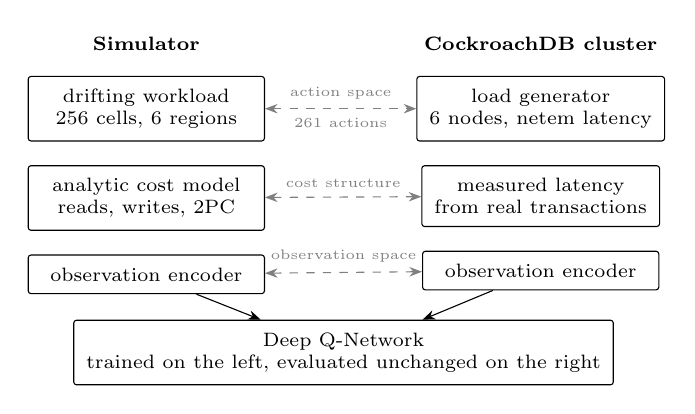
\begin{tikzpicture}[
  node distance=3mm,
  box/.style={draw, rounded corners=1pt, align=center, font=\scriptsize,
              minimum width=30mm, inner sep=1.6mm},
  title/.style={font=\scriptsize\bfseries},
  parity/.style={<->, >={Stealth[length=1.6mm]}, dashed, gray},
  note/.style={font=\tiny, gray, align=center}
]

% Left column: the simulator.
\node[title] (simtitle) {Simulator};
\node[box, below=2mm of simtitle] (simwork) {drifting workload\\256 cells, 6 regions};
\node[box, below=of simwork] (simcost) {analytic cost model\\reads, writes, 2PC};
\node[box, below=of simcost] (simobs) {observation encoder};

% Right column: the real cluster.
\node[title, right=26mm of simtitle] (clutitle) {CockroachDB cluster};
\node[box, below=2mm of clutitle] (cluwork) {load generator\\6 nodes, netem latency};
\node[box, below=of cluwork] (clucost) {measured latency\\from real transactions};
\node[box, below=of clucost] (cluobs) {observation encoder};

% The three parity constraints.
\draw[parity] (simwork) -- node[note, above] {action space} node[note, below] {261 actions} (cluwork);
\draw[parity] (simcost) -- node[note, above] {cost structure} (clucost);
\draw[parity] (simobs) -- node[note, above] {observation space} (cluobs);

% The agent, underneath, moving left to right.
\node[box, below=6mm of $(simobs)!0.5!(cluobs)$, minimum width=62mm]
  (agent) {Deep Q-Network\\trained on the left, evaluated unchanged on the right};
\draw[->, >={Stealth[length=1.6mm]}] (simobs) -- (agent);
\draw[->, >={Stealth[length=1.6mm]}] (cluobs) -- (agent);

\end{tikzpicture}
\caption{The two halves of the system and the three things that must agree
between them. The agent is trained against the simulator, which is fast and
cheap, and evaluated without further training on the cluster, which is slow and
real. Transfer is
only meaningful if the observation space, the action space and the cost
structure are the same on both sides.}
\label{fig:architecture}
\end{figure}

% STATUS: WRITTEN, 15 November 2026, against replication factor 3 and strong
% reads throughout. Every number is transcribed from results/recorded/*.csv or
% from the run directories under results/runs/, and every row in those files
% names the run it came from. Objective costs are computed from the recorded
% latency, movement and imbalance with Eq. (1), never by hand from a figure.

\section{Evaluation}

The evaluation answers five questions, in order. Does it matter on real
hardware where a shard's leaseholder sits? Is the gain from moving data a
gain from \emph{choosing} where to move it? How does the room available to a
better policy change as the workload moves faster? Does the learned policy use
that room in simulation? And does what it learned survive the move to a real
cluster?

% ---------------------------------------------------------------------
\subsection{Setup}

The simulated cluster has six regions, one node per region, replication
factor three, and a keyspace of 256 cells from which shards are built. An
episode is 200 decision windows. At each window the policy sees the
per-region read and write counts from the window just finished and issues one
action; the environment then charges it for the latency its placement
produced and for the data any move carried. Reads are strong: they are served
by the leaseholder, which is how the cluster serves a read that is not marked
as stale, so the simulator and the cluster price a read the same way.

Every policy runs through the same episode loop. The policies are static hash partitioning, random relocation, the
reactive heuristic that follows the traffic, a co-location planner modeled on
Lion~\cite{lion2024}, and the learned policy. The Lion-style planner re-plans
every ten windows: it groups shards that are accessed together, places each
group on one region by a cost model that prefers moving a lease over copying
data, and then rebalances load. Beside them sits a per-window bound: the
lowest latency reachable by relocating every lease for free, each window,
\emph{at the shard boundaries the episode started with}. It is not a global
optimum. A policy that moves replicas or splits shards can score below it.

The agent minimises a single cost, which is the quantity it is judged on
throughout:
%
\begin{equation}
c = \frac{\ell}{100} \;+\; w \cdot \frac{g}{2000} \;+\; 0.10 \cdot b
\label{eq:objective}
\end{equation}
%
where $\ell$ is mean transaction latency in milliseconds, $g$ is gigabytes
moved over the episode, $b$ is load imbalance, and $w$ is the migration
weight, 0.30 unless stated. Latency is what we want low, moving data is
charged for, and concentrating the workload on one node is charged for
separately, so that a policy cannot win on latency by overloading a single
region. Migration is expressed as a fraction of the dataset, so the 60\,GB
simulator and the 1\,GB cluster score the same physical move identically.

The agent is a Deep Q-Network with invalid actions masked both at selection
and in the bootstrap target, and three-step returns, so that a move is
credited with the latency it saves in the windows after it. Masking removes
the inapplicable actions that dominated an earlier unmasked agent; across the
runs reported here the inapplicable share is 0.0\%. Each training run takes
$10^6$ steps at volatility 4.

Two seed blocks appear and are never mixed in one table. The volatility sweep
uses seeds 0 to 7. Agent evaluations use held-out seeds 2000 to 2007, which
the training configuration refuses to overlap with its training seeds.

The cluster has six CockroachDB nodes in containers with inter-region
round-trip times injected by \texttt{netem}, on a four-core GitHub Actions
runner, replication factor three. A harness executes each action as a
synchronous relocation statement, reads the resulting placement back from the
database, and only then times $N=200$ transactions issued from per-region
connections. $N$ was chosen by measuring the standard error of the mean
latency, which is about 1 to 2\,ms per episode at that size. Before any
measurement the harness waits until every range has three voters and then
freezes the database's own rebalancer, so the placement under test is the one
the policy chose.

% ---------------------------------------------------------------------
\subsection{Q1: placement changes latency on real hardware}

The gate runs the same transactions twice on the cluster: once with the
leaseholders for the keys involved gathered in the region issuing them, and
once with those leaseholders spread across regions
(Table~\ref{tab:cluster}, Fig.~\ref{fig:cluster}).

\begin{table}[t]
\caption{Cluster gate, replication factor 3, $N=200$ transactions per arm.
Source: \texttt{results/recorded/cluster.csv}.}
\label{tab:cluster}
\centering
\begin{tabular}{lrr}
\toprule
Leaseholders & p50 (ms) & p95 (ms) \\
\midrule
co-located &  293.6 &  441.7 \\
spread     & 1059.0 & 1779.5 \\
\bottomrule
\end{tabular}
\end{table}

\begin{figure}[t]
\centering
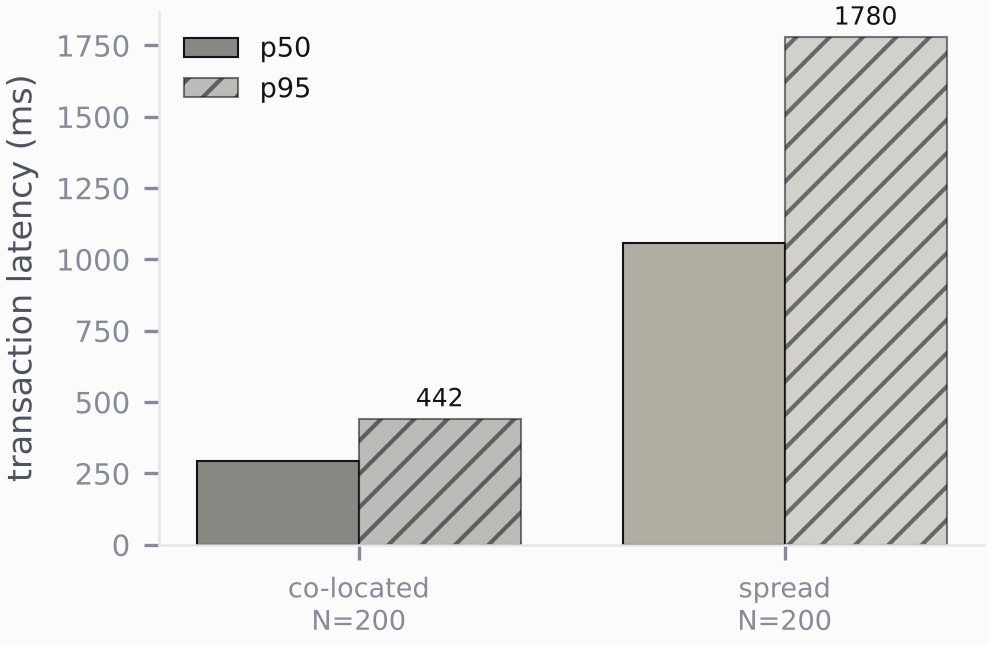
\includegraphics[width=\columnwidth]{cluster.png}
\caption{Co-located against spread leaseholders on the real cluster,
replication factor 3. The difference is far larger than the measurement
noise, which is all this experiment is asked to establish.}
\label{fig:cluster}
\end{figure}

The p95 gap is 1337.8\,ms, with a bootstrap 95\% interval of
[1168.5, 1407.8]\,ms. Placement is worth a great deal on real hardware, which
is the assumption the rest of the work rests on.

Two qualifications belong with that number. First, ``co-located'' means the
leases, not the data. With one node per region the three voters sit in three
regions, so every write still pays a cross-region quorum, which is why the
co-located p50 is 293.6\,ms rather than single digits. What the gate isolates
is the leaseholder effect, which is exactly what the \textsc{move\_lease}
action controls. Second, the co-located arm places every lease on one node,
so it is the arm most exposed to that node saturating. It did not: the
leaseholder node averaged 15.7\% of one core, and the arm's median latency
did not drift across the run. Earlier pilots that suggested saturation had
run on a cluster that had not finished replicating, and are not reported.

% ---------------------------------------------------------------------
\subsection{Q2: the gain comes from choosing, not from moving}

\begin{table}[t]
\caption{Volatility sweep. Mean latency (ms) and data moved per episode
(GB), eight seeds per value, seed block 0 to 7. Source:
\texttt{results/recorded/sweep.csv}.}
\label{tab:sweep}
\centering
\small
\begin{tabular}{lrrrrrr}
\toprule
Vol. & Static & Random & Follow & Lion & Bound & Follow GB \\
\midrule
0.5 & 196.8 & 196.4 & 117.0 & 183.0 & 118.7 & 322.5 \\
1.0 & 196.3 & 201.6 & 119.8 & 181.7 & 118.0 & 632.6 \\
2.0 & 195.5 & 201.6 & 137.4 & 173.3 & 111.5 & 900.2 \\
4.0 & 196.1 & 203.0 & 160.4 & 177.8 & 102.8 & 873.7 \\
\bottomrule
\end{tabular}
\end{table}

The random baseline separates two explanations that are easy to confuse. It
relocates data without looking at the traffic. Across the sweep in
Table~\ref{tab:sweep} it moves 162.7\,GB per episode and ends between 196.4
and 203.0\,ms, no better than doing nothing and at higher volatility slightly
worse. The heuristic, at volatility 1, reaches 119.8\,ms, 39.0\% faster than
static hashing. Movement by itself buys nothing; everything is in the choice
of destination. That is why the problem is a decision problem, and why a
learned policy is a sensible thing to attempt.

% ---------------------------------------------------------------------
\subsection{Q3: the room for a better policy grows with volatility}

Volatility controls how fast the geographic centre of the workload drifts
between windows. Table~\ref{tab:sweep} and Fig.~\ref{fig:sweep} sweep it over
a factor of eight.

Static hashing is flat, 195.5 to 196.8\,ms. It never tracked the workload, so
it does not degrade as the workload moves faster. The bound improves, from
118.7 to 102.8\,ms, because a more volatile workload is a more sharply
concentrated one, and a concentrated workload is easier to serve if the data
is in the right place. Faster drift makes the problem harder for a policy and
easier for an oracle.

The heuristic goes the other way: 117.0\,ms rising to 160.4\,ms, whilst the
data it moves rises from 322.5\,GB to about 900\,GB. Its advantage over static hashing falls from
40.6\% to 18.2\%. A rule that reacts to the window just finished is chasing a
target that has already moved, and under fast drift much of what each move
buys has expired by the time it lands.

\begin{figure*}[t]
\centering
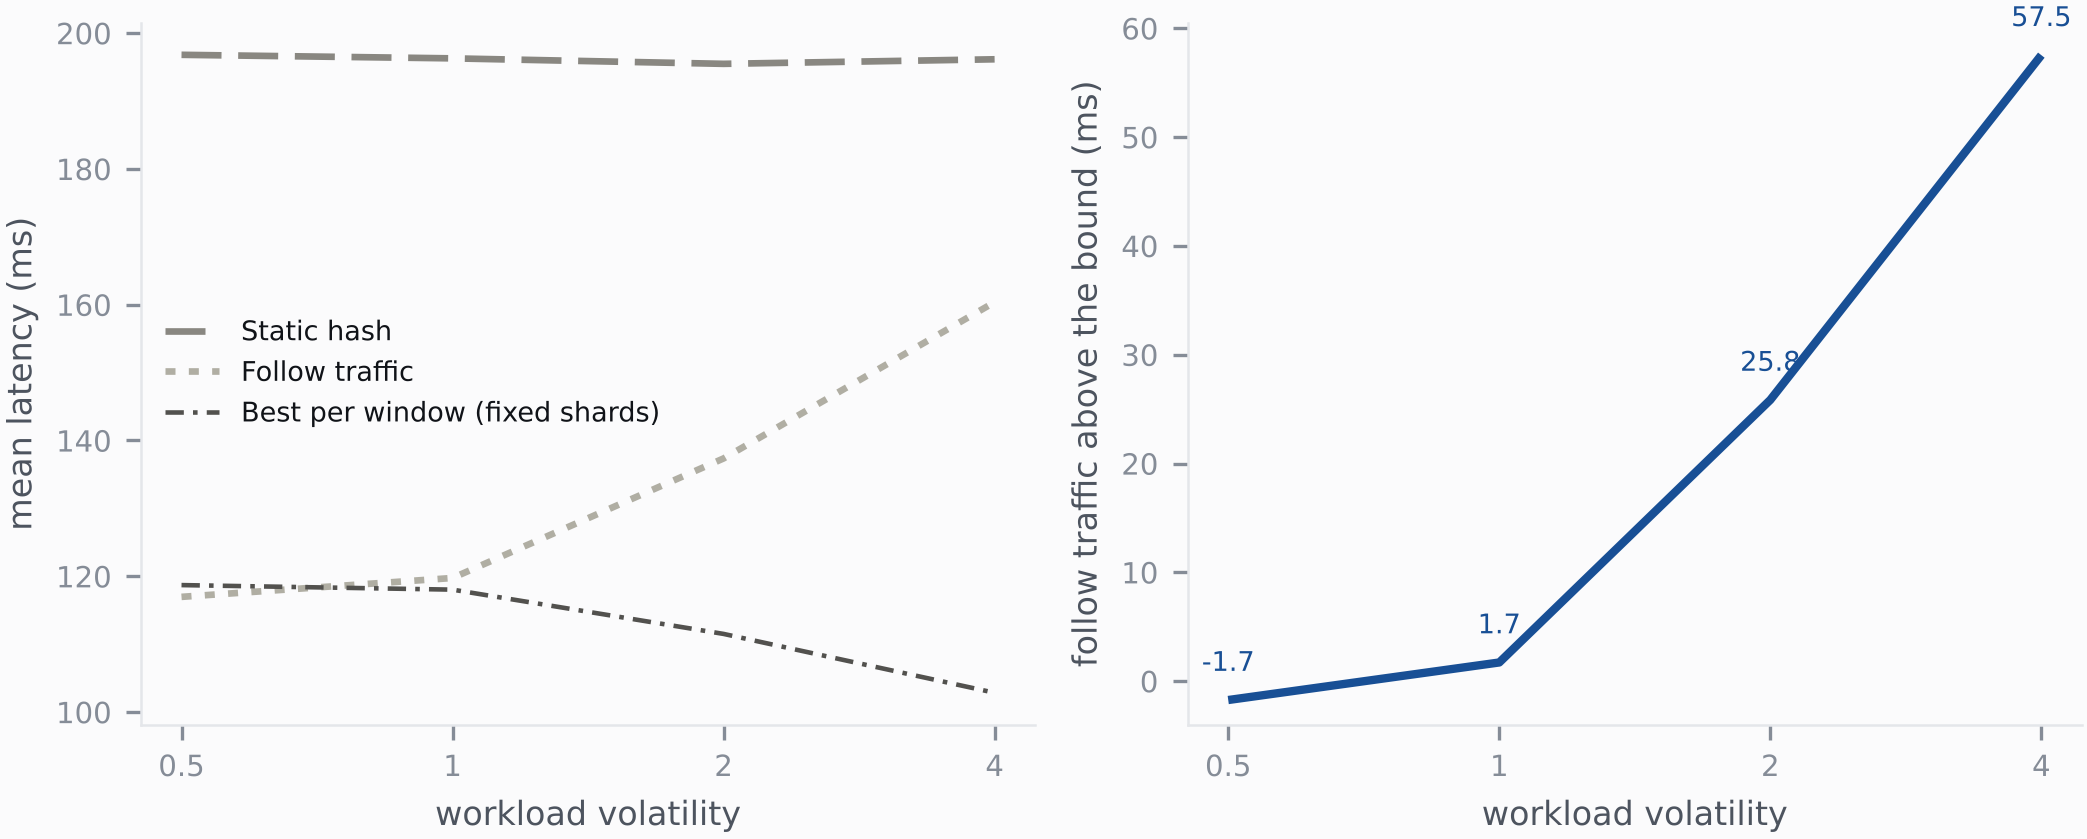
\includegraphics[width=\textwidth]{sweep.png}
\caption{Left: latency against volatility for static hashing, the reactive
heuristic and the per-window bound. Right: the heuristic's distance above the
bound, the room available to a better policy. Seed block 0 to 7.}
\label{fig:sweep}
\end{figure*}


The gap between the heuristic and the bound is $-1.7$\,ms at volatility 0.5,
1.7\,ms at volatility 1, 25.9\,ms at 2 and 57.5\,ms at 4, where it is 36\% of
the heuristic's own latency. At slow drift the heuristic is slightly
\emph{below} the bound, because it moves replicas as well as leases and the
bound moves leases only. Under slow drift, then, a reactive rule is already as
good as the reference, and there is nothing worth learning. Under fast drift
there is a great deal. The case for a learned policy is conditional on
volatility, and the condition is measured rather than assumed. The
Lion-style planner, which re-plans on a fixed period and moves little data
(15 to 24\,GB), sits between static hashing and the heuristic at every
setting.

% ---------------------------------------------------------------------
\subsection{Q4: in simulation the agent trades latency for movement}

Table~\ref{tab:agent} reports four agents trained at volatility 4 from
different learner seeds, evaluated on held-out seeds 2000 to 2007 against
the baselines on the same seeds.

\begin{table}[t]
\caption{Held-out seeds 2000 to 2007, volatility 4, $w=0.30$. Agent rows are
four learner seeds. Source: \texttt{results/recorded/heldout-rf3.csv}.}
\label{tab:agent}
\centering
\begin{tabular}{lrr}
\toprule
Policy & ms & GB moved \\
\midrule
Agent, learner seed 1 & 163.2 & 117.8 \\
Agent, learner seed 2 & 170.7 & 278.1 \\
Agent, learner seed 3 & 162.7 & 121.7 \\
Agent, learner seed 4 & 166.9 & 216.7 \\
\addlinespace
Static hash   & 192.1 &   0.0 \\
Random        & 195.5 & 134.6 \\
Follow traffic& 148.8 & 867.7 \\
Lion-style    & 180.0 &  28.8 \\
Bound         &  91.0 &   0.0 \\
\bottomrule
\end{tabular}
\end{table}

On every learner seed the agent is faster than static hashing, by 13.7\% on
average (165.9 against 192.1\,ms), and faster than the Lion-style planner by
14.1\,ms. It is 17.1\,ms slower than the heuristic and moves 21\% of the
heuristic's data (183.6 against 867.7\,GB on average). It buys its latency
mostly with lease moves, which carry no data: on the cluster episode in Q5,
131 of its 200 actions moved a lease, 55 moved a replica and 14 split a
shard.

Under the objective the comparison with the heuristic is close and goes
against the agent. With the latency and migration terms alone, at $w=0.30$,
the four agents score 1.646 to 1.749 against the heuristic's 1.618; the
imbalance term was not recorded for the agent runs and is omitted from both
sides here. The agent does not beat the heuristic on the objective it was
trained on.

How this verdict depends on the price of movement is the subject of
Table~\ref{tab:weight}. The policies' trajectories are fixed; only the weight
used to score them changes. In simulation, the agent's cost falls below the
heuristic's once $w$ exceeds 0.50, and stays below the Lion-style planner's
until $w$ reaches 1.82. Over that whole band the learned policy is the
cheapest of the four. This is a rescoring, not a retraining: an agent trained
at a higher weight would behave differently, and that experiment has not been
run.

\begin{table}[t]
\caption{Objective cost as the migration weight $w$ varies, with each
policy's behavior fixed. Simulator: held-out seeds, mean of the four agents,
imbalance omitted. Cluster: one episode per policy, full
Eq.~\eqref{eq:objective}. Lowest in each row in bold.}
\label{tab:weight}
\centering
\small
\begin{tabular}{llrrrr}
\toprule
 & $w$ & Agent & Follow & Lion & Static \\
\midrule
Simulator & 0.0 & 1.659 & \textbf{1.488} & 1.800 & 1.921 \\
          & 0.3 & 1.686 & \textbf{1.618} & 1.804 & 1.921 \\
          & 0.6 & \textbf{1.714} & 1.748 & 1.808 & 1.921 \\
          & 1.0 & \textbf{1.751} & 1.922 & 1.814 & 1.921 \\
\addlinespace
Cluster   & 0.0 & 2.008 & \textbf{1.775} & 2.036 & 2.103 \\
          & 0.3 & 2.027 & \textbf{1.890} & 2.041 & 2.103 \\
          & 0.6 & 2.046 & \textbf{2.006} & 2.045 & 2.103 \\
          & 1.0 & 2.072 & 2.160 & \textbf{2.051} & 2.103 \\
\bottomrule
\end{tabular}
\end{table}

Training has plateaued rather than run short: held-out latency stays between
about 160 and 190\,ms from step 50{,}000 to $10^6$, and in three of four runs
the best checkpoint fell before step 170{,}000. The bound, at 91.0\,ms,
remains far away.

% ---------------------------------------------------------------------
\subsection{Q5: the ranking carries over to the cluster}

The agent from the third learner seed, unchanged, was run on the cluster for
a full 200-window episode on workload seed 2000, alongside follow, Lion-style
and static, one episode each (Table~\ref{tab:clustereval}). Every episode
passed the harness checks, with no suspect or divergent step.

\begin{table}[t]
\caption{One 200-window episode per policy on the cluster, workload seed
2000, volatility 4. Simulator column: the same seed and settings. Source:
\texttt{results/recorded/cluster-eval.csv}.}
\label{tab:clustereval}
\centering
\small
\begin{tabular}{lrrrrr}
\toprule
Policy & Cluster ms & Sim.\ ms & GB & Imbal. & Cost \\
\midrule
Follow     & 167.2 & 148.1 & 771.6 & 1.024 & 1.890 \\
Agent      & 192.8 &   --  & 127.5 & 0.801 & 2.027 \\
Lion-style & 191.6 & 153.0 &  30.0 & 1.202 & 2.041 \\
Static     & 206.2 & 182.4 &   0.0 & 0.416 & 2.103 \\
\bottomrule
\end{tabular}
\end{table}

The order under the objective, follow, agent, Lion-style, static, is the
order the simulator gives. The agent is 13.4\,ms (6.5\%) faster than static
hashing and 25.6\,ms slower than the heuristic, moving 16.5\% of its data.
Against the Lion-style planner the latency difference, 1.2\,ms, is inside
the episode's sampling error; the agent's lower cost comes from lower
imbalance.

The simulator's errors are systematic rather than random. For the two
policies all of whose actions were applied, the cluster is slower by a
steady margin: 23.7\,ms (13.0\%) for static hashing and 19.1\,ms (12.9\%)
for the heuristic, whilst the data moved agrees to the decimal. A constant
offset of this kind does not change a ranking, which is what transfer
requires.

The Lion-style planner lost most in transfer, 38.6\,ms. Twenty of its 200
actions were refused, all lease moves, each with the database's reason that
the target ``may need a Raft snapshot''. The planner moves a replica and,
in the next window, moves the lease onto it; CockroachDB will not transfer a
lease to a replica it cannot confirm has caught up. The simulator has no such
rule. The harness records a refused action as refused rather than scoring it
as applied.

The cluster's single episode also changes the weight analysis
(Table~\ref{tab:weight}). On seed 2000 the agent is never the cheapest
policy: the heuristic leads up to $w=0.71$ and the Lion-style planner beyond
it. Seed 2000 is a favorable seed for Lion-style co-location (153.0\,ms in
simulation against its eight-seed mean of 180.0\,ms), so this is one seed
rather than a contradiction, but it is the only cluster evidence there is.

% ---------------------------------------------------------------------
\subsection{Threats to validity}

The simulator's cost model is analytic, and the cluster runs on one host with
\texttt{netem} latency and no injected jitter or loss. Q1 and Q5 establish that placement
matters on hardware and that the simulator ranks policies as the cluster
does on one seed; they do not establish that its magnitudes are right, and
it is about 13\% optimistic where it can be compared.

The cluster results rest on one episode per policy and one workload seed.
The within-episode sampling error is 1 to 2\,ms, but there is no interval
across workload seeds, and none across learner seeds on the cluster.

The agent's imbalance was not recorded in the simulator runs, so the
simulator rows of Table~\ref{tab:weight} omit that term for every policy.
The cluster rows include it.

The weight analysis rescales fixed trajectories. It shows where the price of
movement changes the verdict; it does not show what an agent trained at that
price would do.

Results at one volatility should not be generalised to another, which Q3
demonstrates. The agent results at volatility 4 say nothing about volatility
1, where the heuristic is already at the reference.

% STATUS: WRITTEN, 15 November 2026, after the Evaluation section, so that it
% describes the result that was measured rather than the one that was hoped
% for.

\section{Conclusion and Future Work}

This paper asked whether a reinforcement learning agent can act as an
autonomous database administrator, re-fragmenting and re-allocating shards
as a workload's geographic center of gravity moves. What it establishes is a
measured problem statement, a cluster that confirms the premise, a learned
policy that makes a different and cheaper trade than the obvious heuristic,
and evidence that the agent's place among the policies carries over from
the simulator to the cluster.

On a real six-node CockroachDB cluster, gathering leaseholders in the
issuing region rather than spreading them changes p95 latency by
1337.8\,ms. A reactive heuristic that follows the traffic is 16.9\,ms above
an exact per-window oracle under slow drift and 75.4\,ms above it under fast
drift,
so the case for a learned policy is conditional on volatility, and this work
measures the condition.

At volatility 4 the agent is 13.7\% faster than static hashing on held-out
seeds and faster than a Lion-style co-location planner on all four learner
seeds, and on average it moves about a fifth of the data the heuristic
moves. It is 17\,ms
slower than the heuristic, and at the migration weight it was trained with
the heuristic still has the lower objective cost. Rescoring the same
behavior shows the verdict turns on the price of movement: in simulation the
agent is the cheapest policy for any migration weight between 0.49 and
2.18. On the cluster, over four workload seeds, the heuristic is cheapest and
the agent second on every seed, 12.6\% faster than static hashing on
average, and the simulator is optimistic by a steady 14\% for static
hashing and the heuristic. The Lion-style planner lost more in transfer,
partly to lease moves the database refused onto replicas that had not yet
caught up, a rule the simulator does not model.

% ---------------------------------------------------------------------
\subsection{Future work}

In the order they should be attempted. Add learner seeds to the cluster
evaluation, so it has an interval, and train an agent with splitting
disabled, to measure what fragmentation adds. Train at the migration weight a
deployment cares about, which the rescoring in Table~\ref{tab:weight} can
suggest but not answer. Teach the simulator the database's refusal rule, or
retry a refused move in the next window. Address the plateau with the other
Rainbow components~\cite{hessel2018rainbow}, and choose the checkpoint on
more evaluation episodes and on the objective rather than latency alone.
Finally, fine-tune on the cluster: the harness already executes actions,
reads placement back and computes the simulator's reward, and at about 15\,s
a step the budget, not the code, is the constraint.


% IEEE requires AI-generated content to be disclosed here, naming the system,
% the sections and the level of use. TODO before submission: add every other
% AI tool used (for example Codex or Gemini) and what it did. Keep it
% anonymous: no names, institution or grant until the camera-ready version.
\section*{Acknowledgment}
\ifanonymous The author(s)\else The author\fi{} used Anthropic's Claude throughout this work: to draft and revise text in
every section, to write and review the simulator, agent and cluster-harness
code, to search for related work, to check every cited source and every
reported number against the recorded runs, and, in separate sessions, to
review the paper adversarially and copy-edit it. \ifanonymous The author(s) reviewed\else The author reviewed\fi{} and edited all of it and
\ifanonymous take\else takes\fi{} full responsibility for the content.

% IEEEtran.bst is not obtainable in this environment, so the build uses
% ieeetr, which ships with texlive base. On Overleaf, change this line to
% IEEEtran.
\bibliographystyle{ieeetr}
\bibliography{references}

\end{document}
